\documentclass[12pt,letterpaper]{article}
\usepackage{graphicx,textcomp}
\usepackage{natbib}
\usepackage{setspace}
\usepackage{fullpage}
\usepackage{color}
\usepackage[reqno]{amsmath}
\usepackage{amsthm}
\usepackage{fancyvrb}
\usepackage{amssymb,enumerate}
\usepackage[all]{xy}
\usepackage{endnotes}
\usepackage{lscape}
\newtheorem{com}{Comment}
\usepackage{float}
\usepackage{hyperref}
\newtheorem{lem} {Lemma}
\newtheorem{prop}{Proposition}
\newtheorem{thm}{Theorem}
\newtheorem{defn}{Definition}
\newtheorem{cor}{Corollary}
\newtheorem{obs}{Observation}
\usepackage[compact]{titlesec}
\usepackage{dcolumn}
\usepackage{tikz}
\usetikzlibrary{arrows}
\usepackage{multirow}
\usepackage{xcolor}
\newcolumntype{.}{D{.}{.}{-1}}
\newcolumntype{d}[1]{D{.}{.}{#1}}
\definecolor{light-gray}{gray}{0.65}
\usepackage{url}
\usepackage{listings}
\usepackage{color}

\definecolor{codegreen}{rgb}{0,0.6,0}
\definecolor{codegray}{rgb}{0.5,0.5,0.5}
\definecolor{codepurple}{rgb}{0.58,0,0.82}
\definecolor{backcolour}{rgb}{0.95,0.95,0.92}

\lstdefinestyle{mystyle}{
	backgroundcolor=\color{backcolour},   
	commentstyle=\color{codegreen},
	keywordstyle=\color{magenta},
	numberstyle=\tiny\color{codegray},
	stringstyle=\color{codepurple},
	basicstyle=\footnotesize,
	breakatwhitespace=false,         
	breaklines=true,                 
	captionpos=b,                    
	keepspaces=true,                 
	numbers=left,                    
	numbersep=5pt,                  
	showspaces=false,                
	showstringspaces=false,
	showtabs=false,                  
	tabsize=2
}
\lstset{style=mystyle}
\newcommand{\Sref}[1]{Section~\ref{#1}}
\newtheorem{hyp}{Hypothesis}

\title{Problem Set 2 \\ \large Applied Stats/Quant Methods 1}
\date{Due: October 14, 2024}
\author{Victor Gomez}

\begin{document}
	\maketitle
	\section*{Instructions}
\begin{itemize}
	\item Please show your work! You may lose points by simply writing in the answer. If the problem requires you to execute commands in \texttt{R}, please include the code you used to get your answers. Please also include the \texttt{.R} file that contains your code. If you are not sure if work needs to be shown for a particular problem, please ask.
	\item Your homework should be submitted electronically on GitHub.
	\item This problem set is due before 23:59 on Monday October 14, 2024. No late assignments will be accepted.

\end{itemize}

	
	\vspace{.5cm}
	\section*{Question 1: Political Science}
		\vspace{.25cm}
	The following table was created using the data from a study run in a major Latin American city.\footnote{Fried, Lagunes, and Venkataramani (2010). ``Corruption and Inequality at the Crossroad: A Multimethod Study of Bribery and Discrimination in Latin America. \textit{Latin American Research Review}. 45 (1): 76-97.} As part of the experimental treatment in the study, one employee of the research team was chosen to make illegal left turns across traffic to draw the attention of the police officers on shift. Two employee drivers were upper class, two were lower class drivers, and the identity of the driver was randomly assigned per encounter. The researchers were interested in whether officers were more or less likely to solicit a bribe from drivers depending on their class (officers use phrases like, ``We can solve this the easy way'' to draw a bribe). The table below shows the resulting data.

\newpage
\begin{table}[h!]
	\centering
	\begin{tabular}{l | c c c }
		& Not Stopped & Bribe requested & Stopped/given warning \\
		\\[-1.8ex] 
		\hline \\[-1.8ex]
		Upper class & 14 & 6 & 7 \\
		Lower class & 7 & 7 & 1 \\
		\hline
	\end{tabular}
\end{table}

First, we load this table as a dataset as follows:

\vspace{.5cm}

\lstinputlisting[language=R, firstline=9, lastline=16]{PS02_Victor_Gomez_24365129.R}  
\begin{verbatim}
> data
      not_stopped bribe_requested stopped
Upper          14               6       7
Lower           7               7       1
\end{verbatim}


\vspace{1cm}

\begin{enumerate}
	
	\item [(a)]
	Calculate the $\chi^2$ test statistic by hand/manually (even better if you can do "by hand" in \texttt{R}).\\
	\\
	The $\chi^2$ test statistic $T_{\chi^2}$ for a sample $y$ of length $n$ is :

	\begin{equation}
		T_{\chi^2}:= \sum_{i=0}^{n}\frac{(y_o,i - y_e,i)^2}{y_e,i}
	\end{equation}

	where $y_e,i$ is the expected value for a given occurence $i$ , $i \in  |[0;n]|$ \\
	and $y_o,i$ is the observed value for a given occurence $i$ , $i \in  |[0;n]|$.\\

	where $\forall i \in |[0,n]|,  y_e,i = \frac{raw\_total*column\_total}{grand\_total}$\\ for a given marginal table.
	
	So, we calculate the following table.
	\newpage
	\begin{table}[h!]
		\centering
		\begin{tabular}{ll | c c c c }
			& & Not Stopped & Bribe requested & Stopped/given warning & Row Total\\
			\\[-1.8ex] 
			\hline \\[-1.8ex]
			Upper class & $y_o$  & 14 & 6 & 7 & 27\\
					& $y_e$  & $\frac{567}{42}$ & $\frac{351}{42}$ & $\frac{216}{42}$  & \\
			Lower class &  $y_o$ & 7 & 7 & 1 &15\\
					& $y_e$  & $\frac{315}{42}$ & $\frac{195}{42}$ & $\frac{120}{42} $ & \\
			Column total &         &21&13&8&42\\
			\hline
		\end{tabular}
	\end{table}		

	I.e. , we have : 	

	\begin{align*}
		T_{\chi^2}: &= \frac{(14 - \frac{567}{42})^2}{\frac{567}{42}} + \frac{(6 -\frac{351}{42})^2}{\frac{351}{42}} + \frac{(7 - \frac{216}{42})^2}{\frac{216}{42}} +  \frac{(7 - \frac{315}{42})^2}{\frac{315}{42}}  + \frac{(7 - \frac{195}{42})^2}{\frac{195}{42}}  +  \frac{(1 - \frac{120}{42})^2}{\frac{120}{42}} \\
		&\approx 3.791168\\
	\end{align*}

	In R, that gives :
	\lstinputlisting[language=R, firstline=19, lastline=42]{PS02_Victor_Gomez_24365129.R}  
	\newpage
	i.e. 
	\begin{verbatim}
	> chi2
	[1] 3.791168
	\end{verbatim}
	 So, that confirms that $T_{\chi^2}=3.791168$

	%\vspace{7cm}

	\item [(b)]
	Now calculate the p-value from the test statistic you just created (in \texttt{R}).\footnote{Remember frequency should be $>$ 5 for all cells, but let's calculate the p-value here anyway.}  What do you conclude if $\alpha = 0.1$?\\
	\\
	For applying a a $\chi^2$ test, we point out that the size of the studied sample is $>30$. Furthermore, We consider that the criterion that each frequency is $>$5 is verified (even if it is faulse here, but the criterion of Cochran is verified i.e. more 80\% of the frequencies are $>5$, which means that it is still acceptable to apply such a test). \\
	
	So we consider the null hypothesis$ \mathcal{H}_0:=\{"Variables\_ are\_independent."\}$	\\

	So, that leads to an aleatory variable $t \leadsto \chi^2((n_{raws}-1)(n_{columns}-1)) = \chi^2(2)$ where $\chi^2$ is the $ \chi^2$ distribution. 
	
	Therefore,  the p-value $p$ is

	\begin{align*}
		p:&=P(t<T_{\chi^2}|\mathcal{H}_0) &\mbox{and $T_{\chi^2}\approx 3.79$} \\
		 &\mbox{ $p\in |[0.1;0.2]|$ because $ F_{\chi^2,2}(0.8)=3.22< T_{\chi^2}< 4.61= F_{\chi^2,2}(0.9)$ }\\
		&\mbox{where $F_{\chi^2,n}$ is the repartition function of the $\chi^2$ distribution with n degrees of freedom, $n\in IN$ }
	\end{align*}	
	This can be refine by linear interpolation, but, we can also use \texttt{R},which gives,
	\lstinputlisting[language=R, firstline=45, lastline=45]{PS02_Victor_Gomez_24365129.R}  
	
	\begin{verbatim}
		> pval
		[1] 0.1502306
	\end{verbatim}

	So, at risk $\alpha=0.1, \mathcal{H}_0$ is not rejected. ($p>\alpha$).

	\newpage
	\item [(c)] Calculate the standardized residuals for each cell and put them in the table below.
	\vspace{1cm}

	The standard residuals $z_{i,j}=\frac{y_{o, (i,j)}-y_{e, (i,j)}}{\sqrt{ y_{e, (i,j)} (1- \frac{ sum_{raw_i}}{sum_{global}})(1- \frac{ sum_{column_j}}{sum_{global}}{})  }} , \forall (i,j) \in |[1,2]|x|[1,3]|$

	\begin{table}[h]
		\centering
		\begin{tabular}{l | c c c }
			& Not Stopped & Bribe requested & Stopped/given warning \\
			\\[-1.8ex] 
			\hline \\[-1.8ex]
			Upper class  & 0.3220306 &-1.641957 &  1.523026 \\
			Lower class & -0.3220306&  1.641957 &-1.523026 \\
			
		\end{tabular}
	\end{table}
	
	In  \texttt{R}, this is calculate with, 
	\lstinputlisting[language=R, firstline=47, lastline=55]{PS02_Victor_Gomez_24365129.R}  
		

	%\vspace{7cm}
	\item [(d)] How might the standardized residuals help you interpret the results?  

	The standardized residuals explain how far a given value is from the expected value, in number of standard deviation. So, the table above, shows that the biggest variations between variables are in categories "Bribe requested" and "Stopped".

\end{enumerate}
%\newpage

\section*{Question 2: Economics}
Chattopadhyay and Duflo were interested in whether women promote different policies than men.\footnote{Chattopadhyay and Duflo. (2004). ``Women as Policy Makers: Evidence from a Randomized Policy Experiment in India. \textit{Econometrica}. 72 (5), 1409-1443.} Answering this question with observational data is pretty difficult due to potential confounding problems (e.g. the districts that choose female politicians are likely to systematically differ in other aspects too). Hence, they exploit a randomized policy experiment in India, where since the mid-1990s, $\frac{1}{3}$ of village council heads have been randomly reserved for women. A subset of the data from West Bengal can be found at the following link: \url{https://raw.githubusercontent.com/kosukeimai/qss/master/PREDICTION/women.csv}\\

\noindent Each observation in the data set represents a village and there are two villages associated with one GP (i.e. a level of government is called "GP"). Figure~\ref{fig:women_desc} below shows the names and descriptions of the variables in the dataset. The authors hypothesize that female politicians are more likely to support policies female voters want. Researchers found that more women complain about the quality of drinking water than men. You need to estimate the effect of the reservation policy on the number of new or repaired drinking water facilities in the villages.
\vspace{.5cm}
\begin{figure}[h!]
	\caption{\footnotesize{Names and description of variables from Chattopadhyay and Duflo (2004).}}
	\vspace{.5cm}
	\centering
	\label{fig:women_desc}
	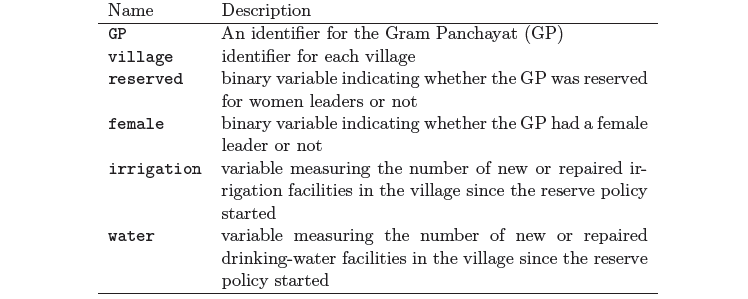
\includegraphics[width=1.1\textwidth]{women_desc.png}
\end{figure}		

\newpage
\begin{enumerate}
	\item [(a)] State a null and alternative (two-tailed) hypothesis. 
	
	We want to anwser if there a correlation between drinking water facilities renewval or reparation and the reservation policy.
	\\ Therefore, a test which can be done is the test of correlation between those two variables, \\
	i.e. considering a nul hypothesis $\mathcal{H}_0 = \{ \rho = 0 \}$ \\
	and an alternative hypothesis $\mathcal{H}_1 = \{ \rho \neq 0 \}$\\
	\\
	In addition, this is a two-tailed hypothesis, since  $\mathcal{H}_1 = \{ \rho < 0 \} \cup \{ \rho > 0 \} $ corresponding to each tail.
		
	%\vspace{6cm}
	\item [(b)] Run a bivariate regression to test this hypothesis in \texttt{R} (include your code!).
	
	First, we load data, and then run a linear regression.
	\lstinputlisting[language=R, firstline=64, lastline=69]{PS02_Victor_Gomez_24365129.R}  
	
	\begin{figure}[h!]\centering
		\caption{\footnotesize Linear regression of Water repair function of Reserved policy }
		\label{fig:plot_2}
		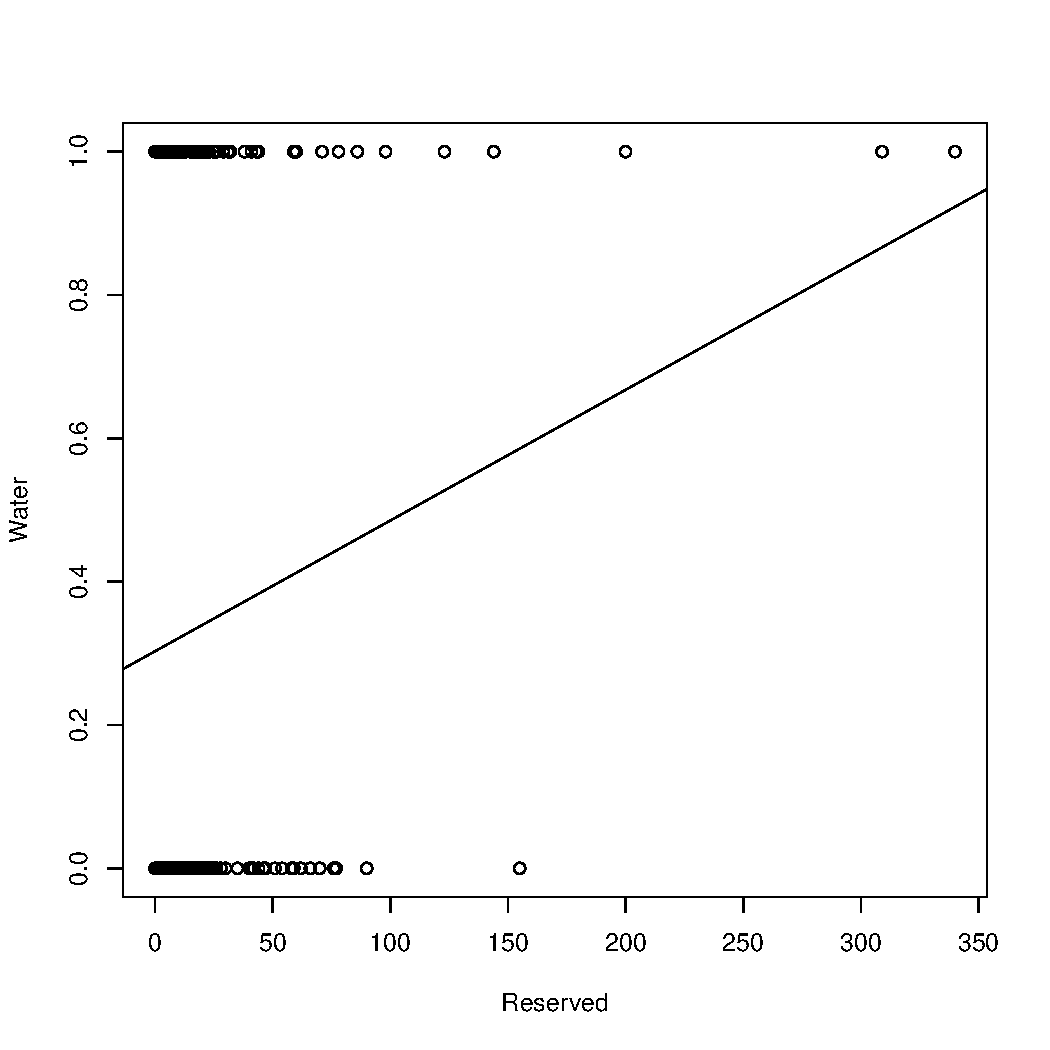
\includegraphics[width=.85\textwidth]{lm.pdf}
	\end{figure}

	In addition, we have the summary:
	\begin{verbatim}
	> summary(model)
		
		Call:
		lm(formula = women$reserved ~ women$water)
		
		Residuals:
		    Min      1Q  Median      3Q     Max 
		-0.5856 -0.3247 -0.3083  0.6602  0.6971 
		
		Coefficients:
		             Estimate Std. Error t value Pr(>|t|)    
		(Intercept) 0.3028613  0.0296247  10.223   <2e-16 ***
		women$water 0.0018240  0.0007782   2.344   0.0197 *  
		---
		Signif. codes:  0 ‘***’ 0.001 ‘**’ 0.01 ‘*’ 0.05 ‘.’ 0.1 ‘ ’ 1
		
		Residual standard error: 0.4696 on 320 degrees of freedom
		Multiple R-squared:  0.01688,	Adjusted R-squared:  0.0138 
		F-statistic: 5.493 on 1 and 320 DF,  p-value: 0.0197
	\end{verbatim}	
	
	We have the$ p-value = 0.0197 < 5\%$ So, the test is statisticly significative.  \\
	But it should be remark the correlation coefficient is $\rho^2=  0.01688$, so there is a statisticly significative small correlation but not null correlation. Indeed, with the given standard error for the slope coefficient ($\sigma = 0.0007782$) we found a confidence interval at 95\% $ CI = |[0.0002676, 0.0033804]| $.\\
	I.e. $0 \notin CI.$a
%	\vspace{6cm}

	\item [(c)] Interpret the coefficient estimate for reservation policy. 

	Here, we have 	 the correlation coefficient $\rho^2=  0.01688$ for the bivariate linear relation between reservation policy and water infrstructure renewval or repair. In other words, that means that only $~1.7\%$ of the variation of the water infrastructure political impact is due to the reservation policy.

\end{enumerate}

\end{document}
